\documentclass[tikz, border=5pt]{standalone}
\usetikzlibrary{patterns}

\begin{document}

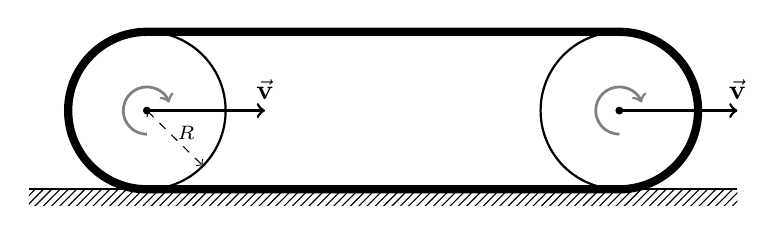
\begin{tikzpicture}

    %% Side view of tank crawler belt
    % Left wheel
    \draw[thick] (-3,0) circle (1);
    \draw[->, line width=1pt] (-3,0) -- (-1.5,0) node[above] {\(\vec{\mathbf{v}}\)};
    \draw[->, line width=1pt, black!50] (-3,-0.3) arc[start angle=270, end angle=20, radius=0.3];
    \draw[<->, dashed] (-3,0) -- (-2.29,-0.7) node[pos=0.7, above] {\scriptsize \(R\)};
    \fill[black] (-3,0) circle (0.05);

    % Right wheel
    \draw[thick] (3,0) circle (1);
    \draw[->, line width=1pt] (3,0) -- (4.5,0) node[above] {\(\vec{\mathbf{v}}\)};
    \draw[->, line width=1pt, black!50] (3,-0.3) arc[start angle=270, end angle=20, radius=0.3];
    \fill[black] (3,0) circle (0.05);

    % Crawler belt
    \draw[line width=3pt] (-3,1) arc[start angle=90,end angle=270,radius=1] -- (3,-1)
    arc[start angle=-90,end angle=90,radius=1] -- cycle;

    % Ground
    \draw[thick] (-4.5,-1) -- (4.5,-1);
    \fill[pattern=north east lines] (-4.5,-1) rectangle (4.5,-1.2);

\end{tikzpicture}

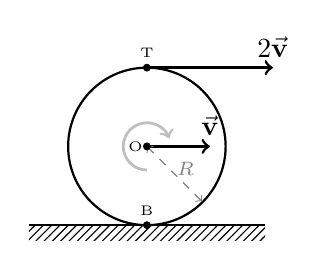
\begin{tikzpicture}

    %% Side view of wheel
    % Left wheel
    \draw[thick] (0,0) circle (1);
    \draw[->, line width=1pt] (0,0) -- (0.8,0) node[above] {\(\vec{\mathbf{v}}\)};
    \draw[->, line width=1pt, black!25] (0,-0.3) arc[start angle=270, end angle=20, radius=0.3];
    \draw[<->, dashed, gray] (0,0) -- (0.7,-0.7) node[pos=0.7, above] {\scriptsize \(R\)};
    \fill[black] (0,0) circle (0.05);
    \node[left, xshift=2] at (0,0) {\tiny O};

    % Ground
    \draw[thick] (-1.5,-1) -- (1.5,-1);
    \fill[pattern=north east lines] (-1.5,-1) rectangle (1.5,-1.2);

    % Bottom
    \fill[black] (0,-1) circle (0.05);
    \node[above] at (0,-1) {\tiny B};

    % Top
    \fill[black] (0,1) circle (0.05);
    \node[above] at (0,1) {\tiny T};
    \draw[->, line width=1pt] (0,1) -- (1.6,1) node[above] {\(2\vec{\mathbf{v}}\)};

\end{tikzpicture}

\end{document}
